\documentclass{article}
\usepackage{graphicx}
\usepackage{amsmath}
\usepackage{subcaption}
\usepackage[margin=1.25in]{geometry}
\usepackage{float}

\author{Fraser Paterson 22258324}
\title{MATH3024 Project}

\begin{document}

\maketitle

\section*{Introduction}

This is the project for Fraser Paterson.
All dynamics were generated via from scipy.integrate.odeint and each call to odeint performed an integral over 10000 time steps.

\section*{Questions}

\subsection*{Question 1}

The system for question 1 is as follows:

$$\dot{x} = \alpha(y - x - f(x))$$
$$\dot{y} = x - y + z$$
$$\dot{x} = -\beta y$$
where
$$f(x) = bx + \frac{1}{2}(a - b)[|x + 1| - |x - 1|]$$
and $\alpha = 10.0, \beta = 14.87, a = -1.27, b = -0.68$

\paragraph{1.a} This is as described in my interem report.

\paragraph{1.b} For an x to x coupling we take a copy of the entire system and add the
difference in the x coordinates, multiplied by the coupling strength: $\sigma$, to both x coordinates
in each respective system. Let each coordinate dynamics
be given by a primed value, hence we have:

$$\dot{x} = \alpha(y - x - f(x)) + \sigma(x' - x)$$
$$\dot{y} = x - y + z\newline$$
$$\dot{x} = -\beta y\newline$$
$$\dot{x'} = \alpha(y' - x' - f(x')) +\sigma(x - x')$$
$$\dot{y'} = x' - y' + z'$$
$$\dot{x'} = -\beta y'$$
where
$$f(x') = bx + \frac{1}{2}(a - b)[|x' + 1| - |x' - 1|]$$
and the parameters remain as above.

See figures 1, 2 and 3 for plots of each respective coordinate dynamics (uncoupled dynamics).

\begin{figure}[H]
\centering
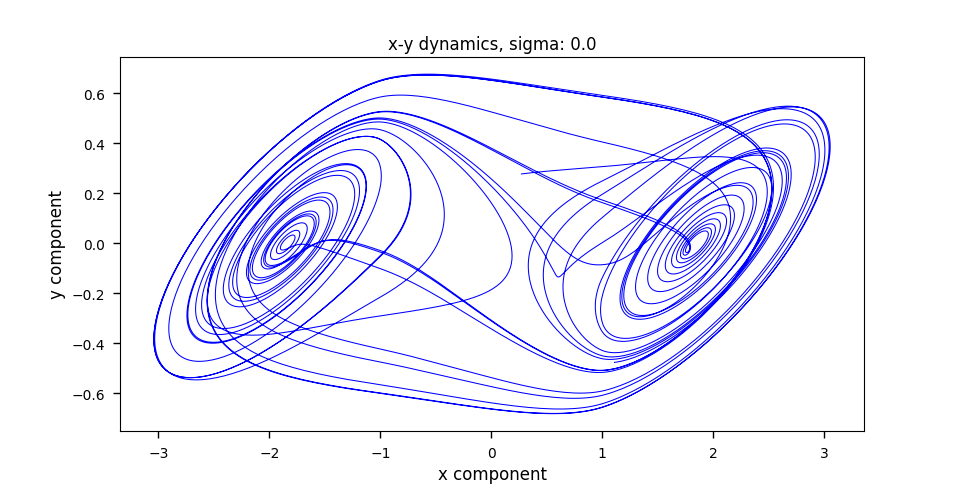
\includegraphics[width = 4in, height = 2in]{dynamics_xy.png}
\caption{x - y dynamics}
\end{figure}

\begin{figure}[H]
\centering
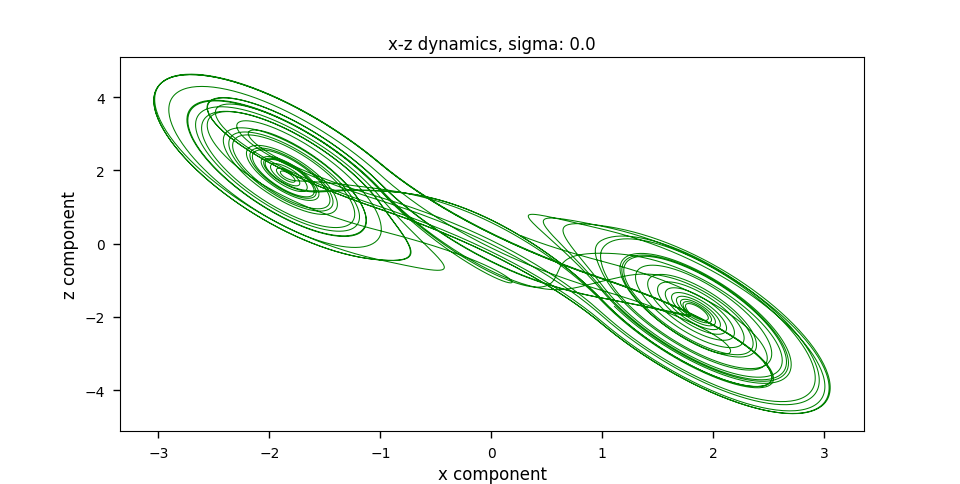
\includegraphics[width = 4in, height = 2in]{dynamics_xz.png}
\caption{x - z dynamics}
\end{figure}

\begin{figure}[H]
\centering
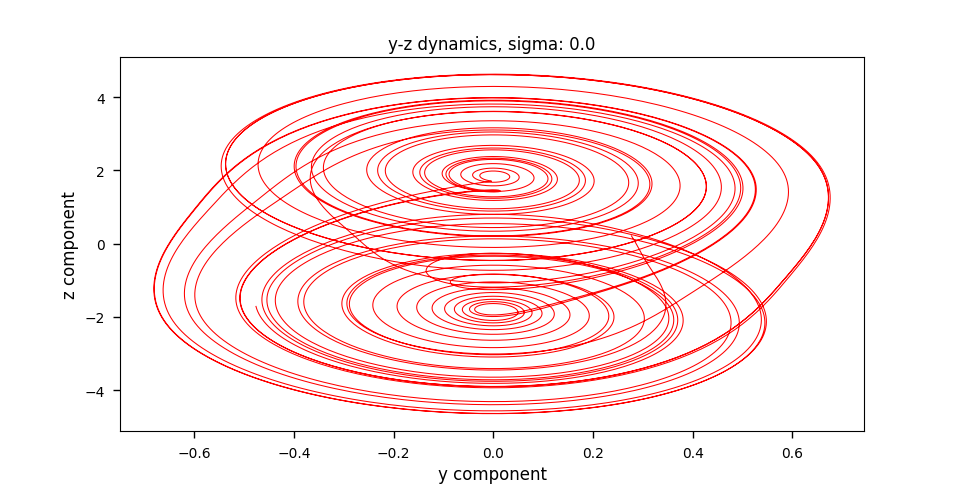
\includegraphics[width = 4in, height = 2in]{dynamics_yz.png}
\caption{y - z dynamics}
\end{figure}

The uncoupled dynamics in time are as follows:

\begin{figure}[H]
\centering
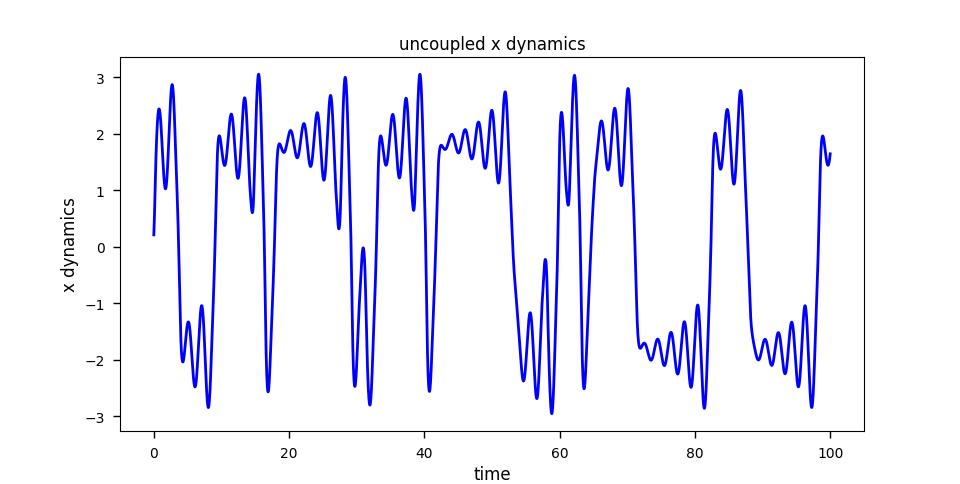
\includegraphics[width = 4in, height = 2in]{x_dynamics_t.png}
\caption{uncoupled x component dynamics}
\end{figure}

\begin{figure}[H]
\centering
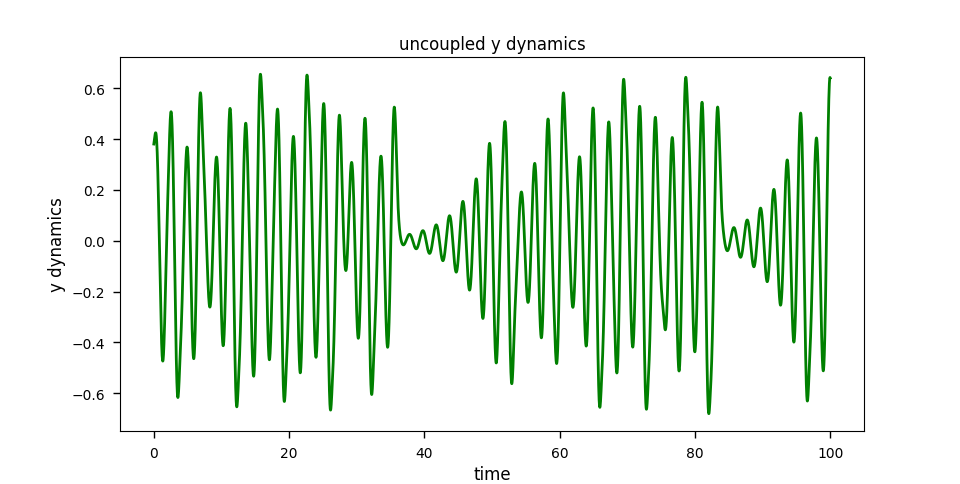
\includegraphics[width = 4in, height = 2in]{y_dynamics_t.png}
\caption{uncoupled y component dynamics}
\end{figure}

\begin{figure}[H]
\centering
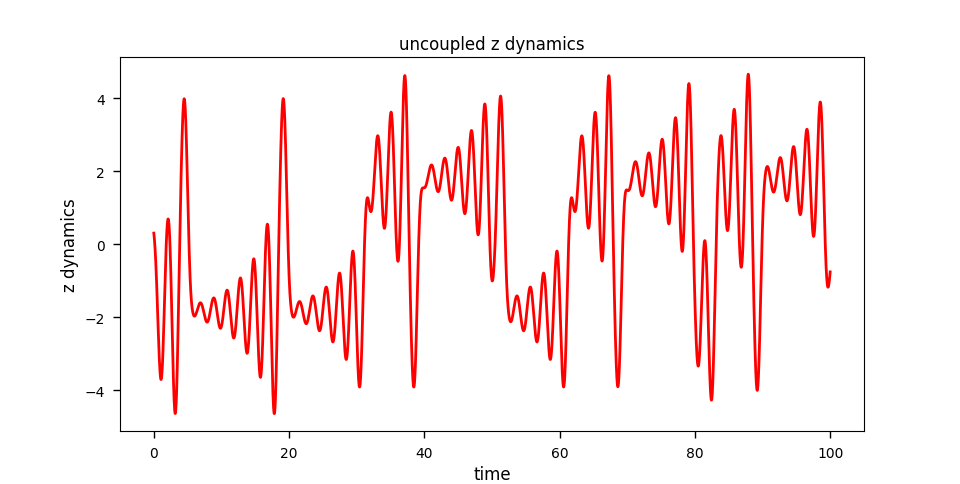
\includegraphics[width = 4in, height = 2in]{z_dynamics_t.png}
\caption{uncoupled z component dynamics}
\end{figure}


To analyse the stability of the coupling for any given $\sigma \in [0, 10.0]$ we define the following
errors in each respective component of the coupled dynamics:

$$e_{x} = x - x'$$
$$e_{y} = y - y'$$
$$e_{z} = z - z'$$

Substituting in each respective expression for x and x' into these error equations, we have:

$$e_{x} = \alpha(e_{y} - e_{x} - (f(x) - f(x'))) - 2\sigma e_{x}$$


Note, that by the intermidiate value theorem $f(x) - f(x') = f'(\eta)(x - x')$ we may express the above as:

$$e_{x} = \alpha(e_{y} - e_{x} - f'(\eta)e_{x}) - 2\sigma e_{x}$$

Now, $f'(\eta)$ = a or b. Hence let $f'(\eta) = \xi$ and so
we have: $e_{x} = (-\alpha - \alpha\xi - 2\sigma)e_{x} + \alpha e_{y}$. Performing a
similar set of substitutions for the y and z errors yields the full error dynamics:

$$e_{x} = (-\alpha - \alpha\xi - 2\sigma)e_{x} + \alpha e_{y}$$
$$e_{y} = e_{x} - e_{y} + e_{z}$$
$$e_{z} = -\beta e_{y}$$

Expressing the error dynamics as a matrix equation:


$$
\begin{pmatrix}
    \dot{e_{x}} \\
    \dot{e_{y}} \\
    \dot{e_{z}} \\
\end{pmatrix} =
\begin{pmatrix}
-\alpha - \alpha\xi - 2\sigma & \alpha & 0\\
1 & -1 & 0\\
0 & -\beta & 0
\end{pmatrix}
\begin{pmatrix}
    e_{x} \\
    e_{y} \\
    e_{z} \\
\end{pmatrix}
$$


Now if we numerically calculate each respective component error and plot this against the coupling strength,
for $\sigma \in [0, 10.0]$, where we take step sizes of 0.01 for $\sigma$ we yield the plots shown in figures 4, 5 and 6. Note, there were no further
changes to the x component error for $\sigma \in (5, 10]$

\begin{figure}[H]
\centering
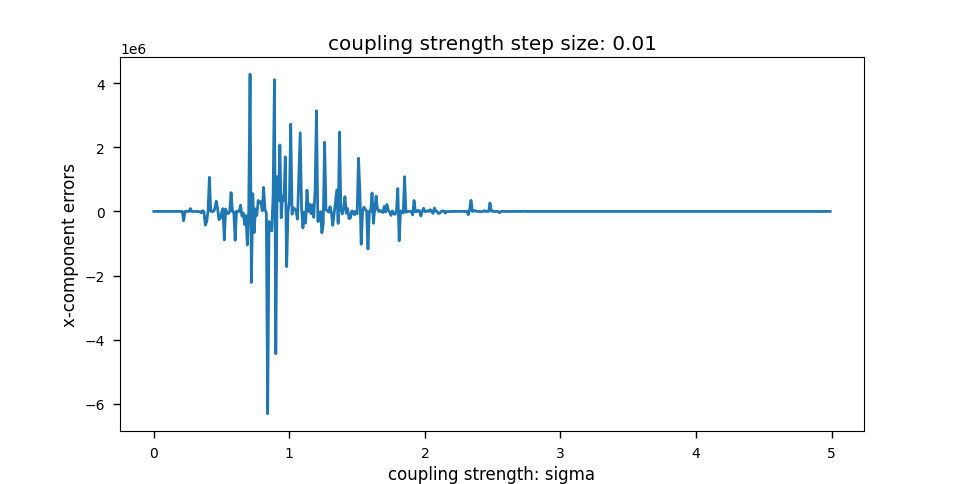
\includegraphics[width = 4in, height = 2in]{x_errors.png}
\caption{x component error dynamics}
\end{figure}

\begin{figure}[H]
\centering
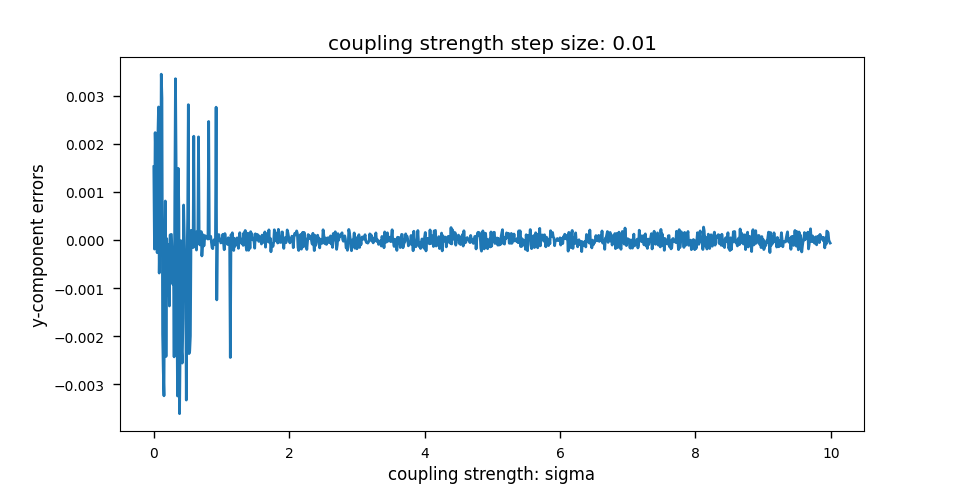
\includegraphics[width = 4in, height = 2in]{y_errors_3.png}
\caption{y component error dynamics}
\end{figure}

\begin{figure}[H]
\centering
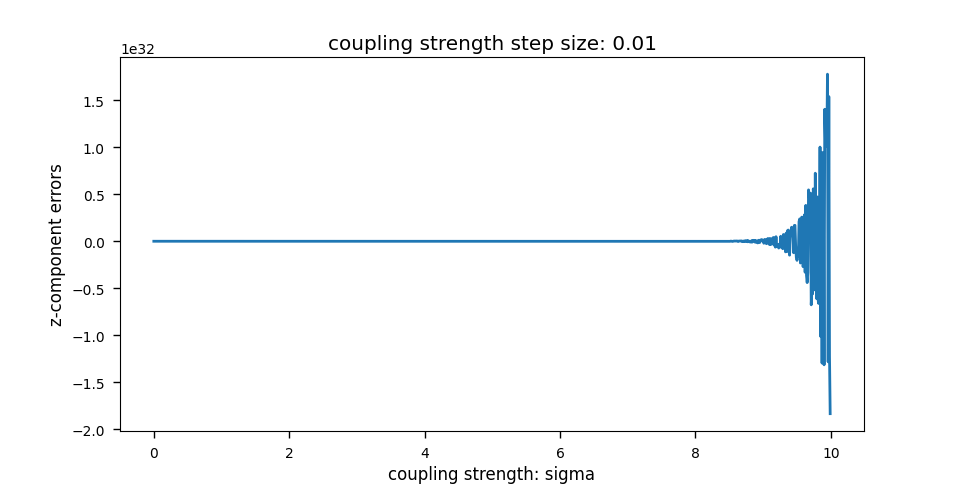
\includegraphics[width = 4in, height = 2in]{z_errors_3.png}
\caption{z component error dynamics}
\end{figure}


Numerically integrating the system of x-x coupled dynamics yields the plots shown in figure 7 to 12.
The plots in navy blue correspond to sigma = 2.6 while those in red correspond to sigma = 2.8.

\begin{figure}[H]
\centering
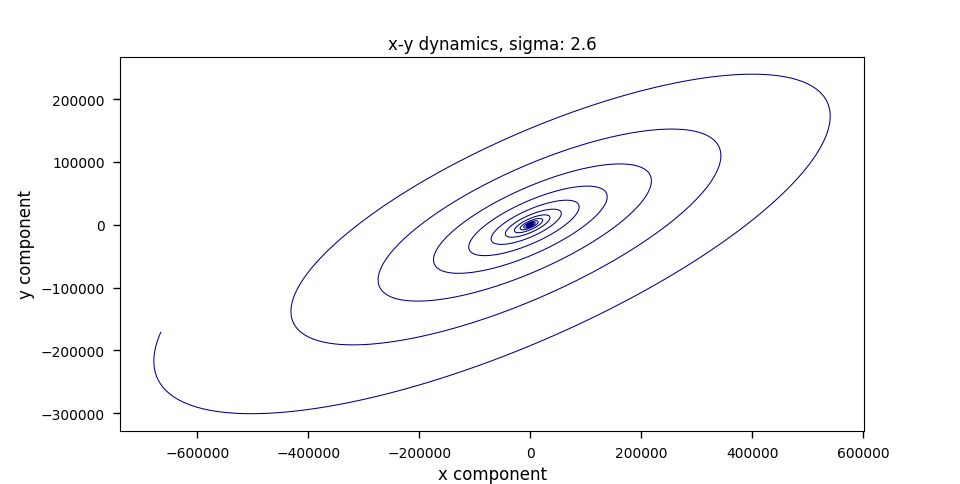
\includegraphics[width = 4in, height = 2in]{x_coupled_s26_xy.png}
\caption{x - y dynamics for x-x coupling}
\end{figure}

\begin{figure}[H]
\centering
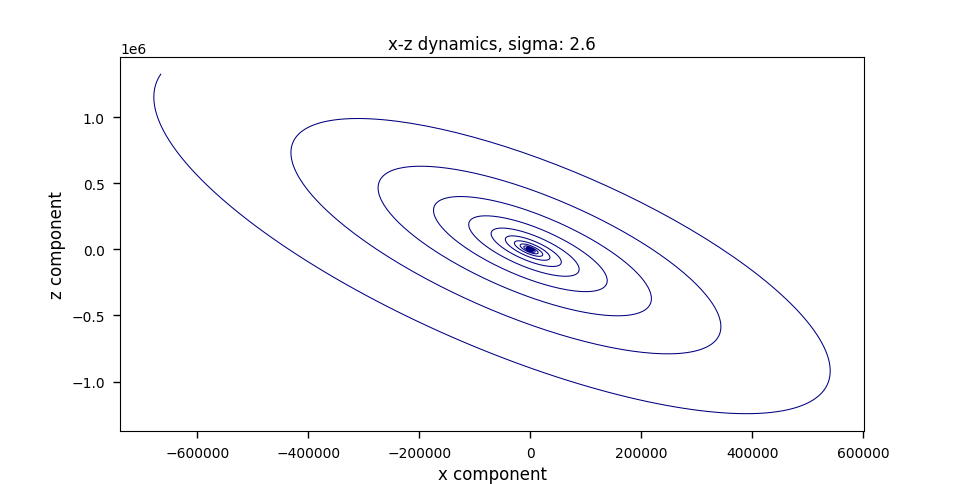
\includegraphics[width = 4in, height = 2in]{x_coupled_s26_xz.png}
\caption{x - z dynamics for x-x coupling}
\end{figure}

\begin{figure}[H]
\centering
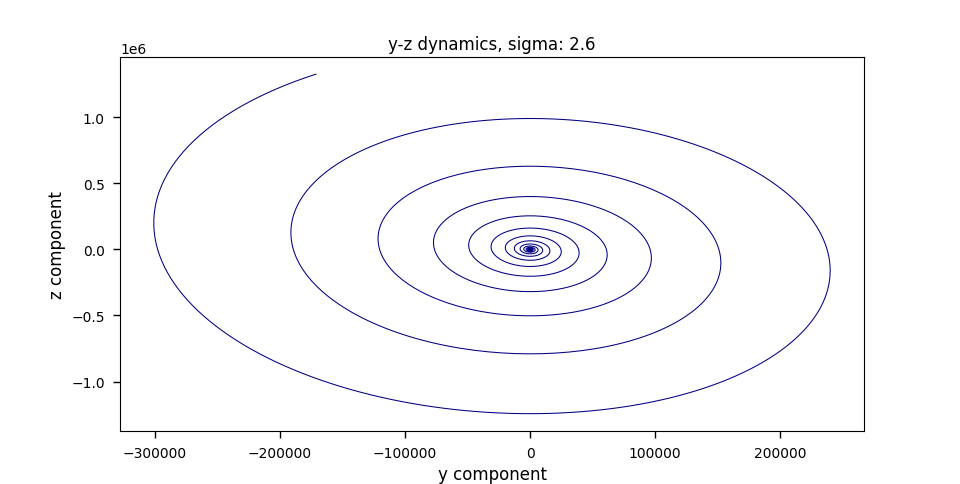
\includegraphics[width = 4in, height = 2in]{x_coupled_s26_zy.png}
\caption{x - z dynamics for x-x coupling}
\end{figure}

\begin{figure}[H]
\centering
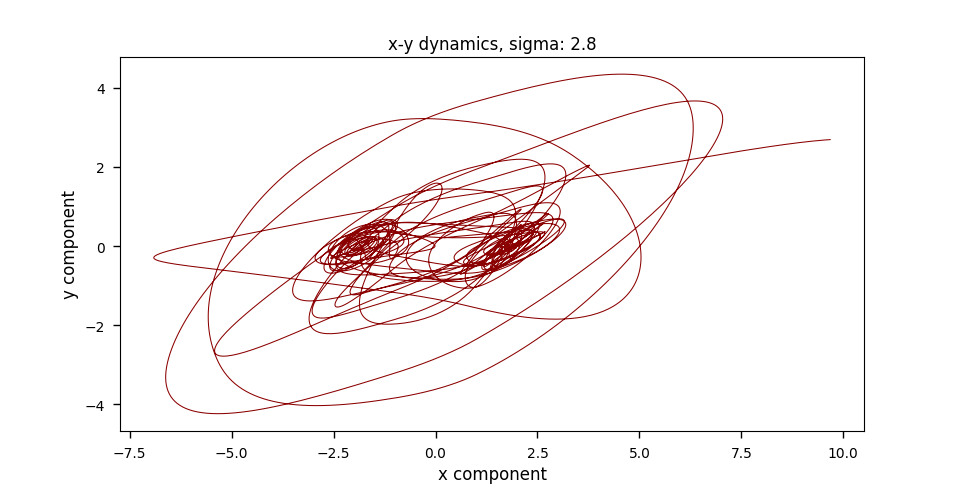
\includegraphics[width = 4in, height = 2in]{x_coupling_s28_xy.png}
\caption{x - y dynamics for x-x coupling}
\end{figure}

\begin{figure}[H]
\centering
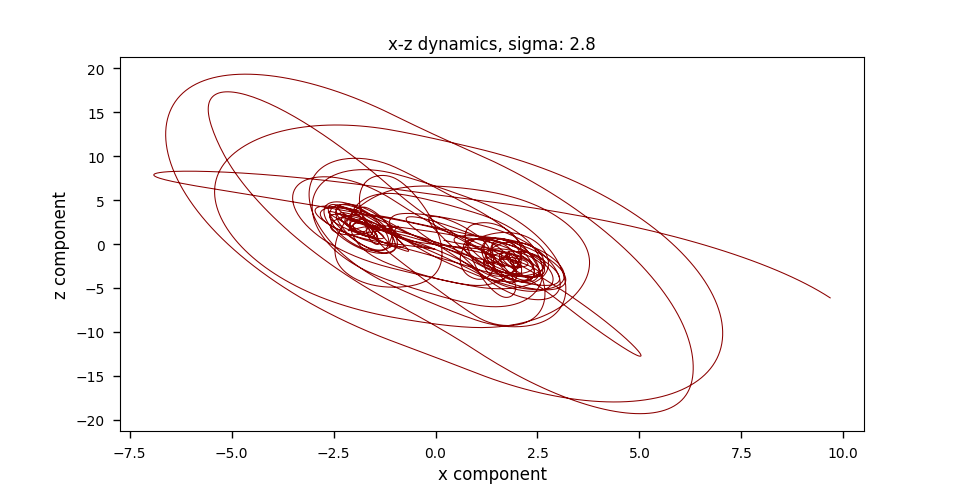
\includegraphics[width = 4in, height = 2in]{x_coupling_s28_xz.png}
\caption{x - z dynamics for x-x coupling}
\end{figure}

\begin{figure}[H]
\centering
\includegraphics[width = 4in, height = 2in]{x_coupling_s28_zy.png}
\caption{x - z dynamics for x-x coupling}
\end{figure}

The dynamics in navy correspond
to an unstable node; as can be seen if we plot the component dynamics in time for $\sigma = 2.6$

\begin{figure}[H]
\centering
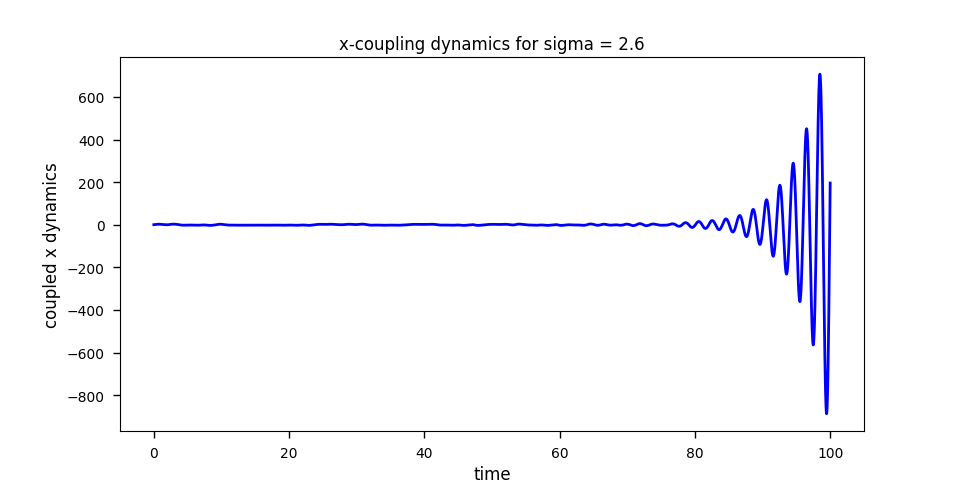
\includegraphics[width = 4in, height = 2in]{x_coupling_x_dynamics_s26.png}
\caption{x component dynamics through time for x-x coupling}
\end{figure}

\begin{figure}[H]
\centering
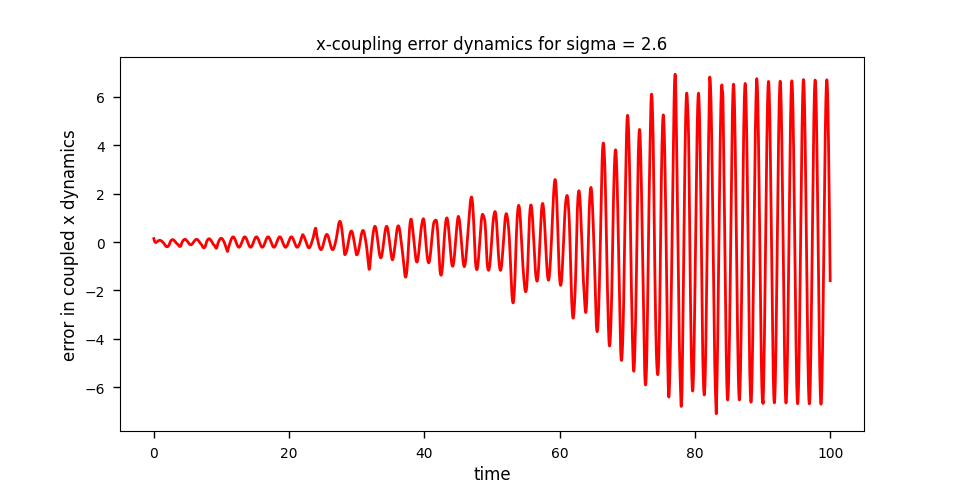
\includegraphics[width = 4in, height = 2in]{x_coupling_x_errors_s26.png}
\caption{x component error dynamics through time for x-x coupling}
\end{figure}

Although the x component error dynamics for $\sigma = 2.8$ is not yet 0, we can see that the error in the x component reaches a maximum and then begins to decrease with time:

\begin{figure}[H]
\centering
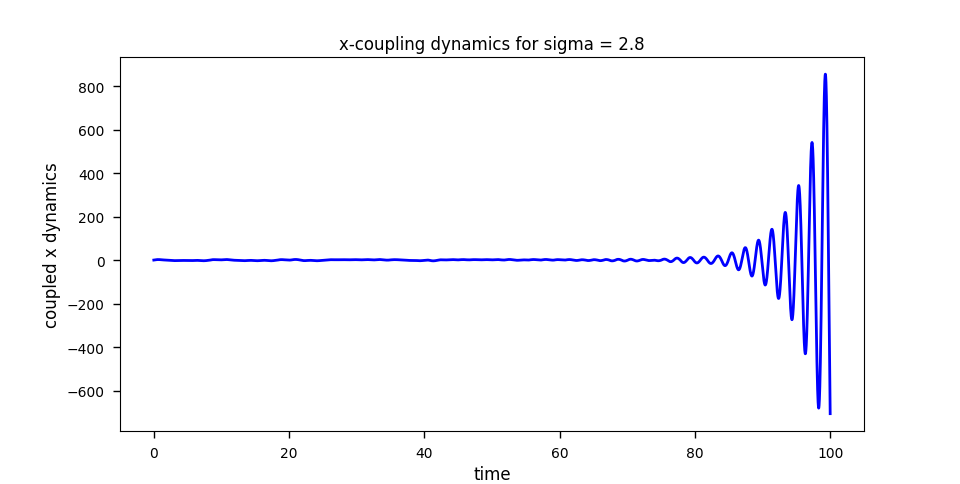
\includegraphics[width = 4in, height = 2in]{x_coupled_x_dynamics_s28.png}
\caption{x component dynamics through time for x-x coupling}
\end{figure}

\begin{figure}[H]
\centering
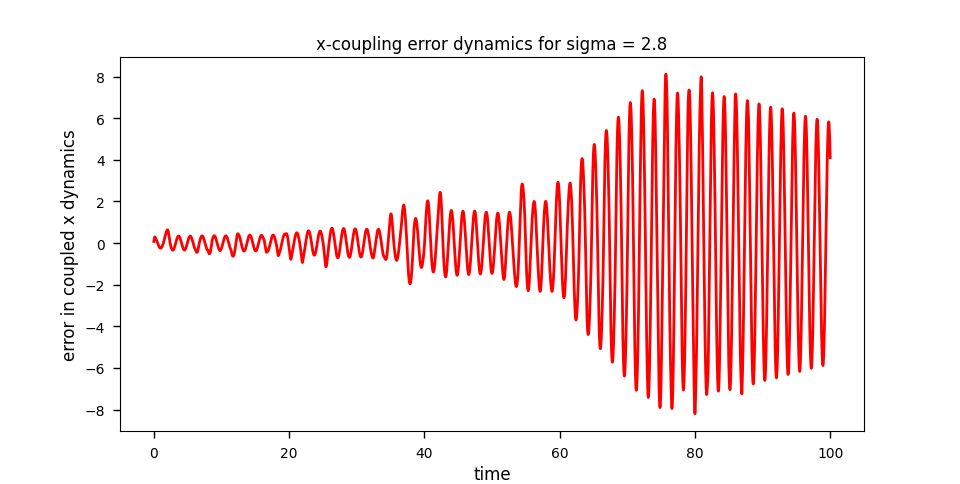
\includegraphics[width = 4in, height = 2in]{x_coupling_x_errors_s28.png}
\caption{x component error dynamics through time for x-x coupling}
\end{figure}

Indeed by $\sigma = 3.9$ at the latest, the error in the x component becomes negligible over the domain displayed:

\begin{figure}[H]
\centering
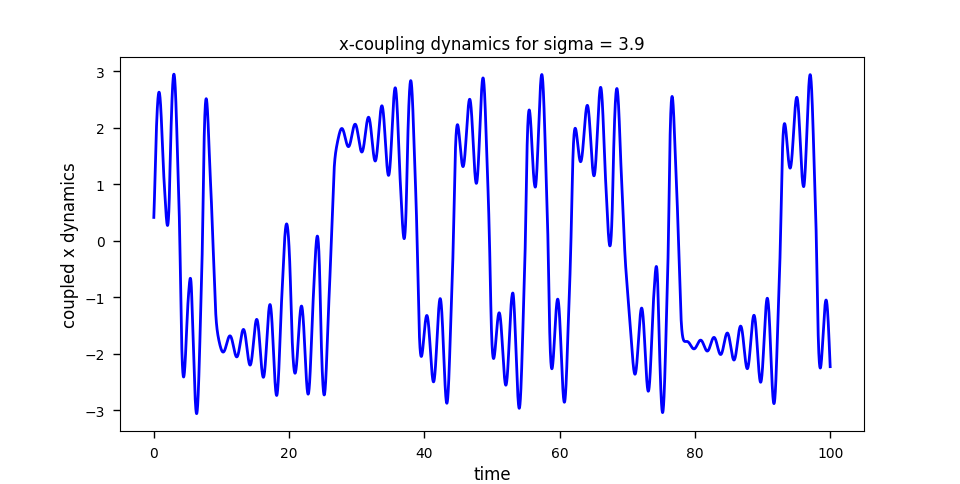
\includegraphics[width = 4in, height = 2in]{x_coupling_x_dynamics_s39.png}
\caption{x component dynamics through time}
\end{figure}

\begin{figure}[H]
\centering
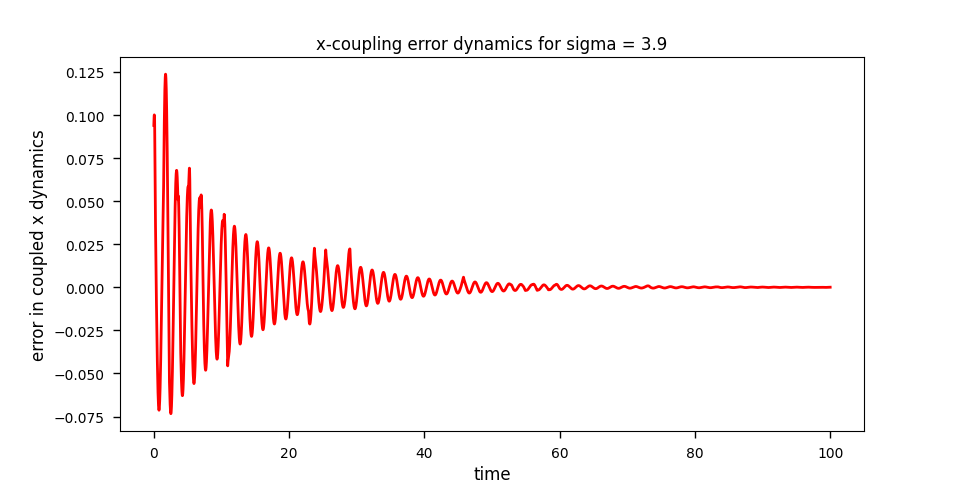
\includegraphics[width = 4in, height = 2in]{x_coupling_x_errors_s39.png}
\caption{x component error dynamics through time}
\end{figure}


\paragraph{1.c} In the case of a y to y and z to z coupling, we perform the same series of operations
as in the above x to x coupling, making sure to add the coupling term to the correct dynamical component

For the y to y coupling we have:

$$\dot{x} = \alpha(y - x - f(x)) $$
$$\dot{y} = x - y + z + \sigma(y - y')$$
$$\dot{x} = -\beta y\newline$$
$$\dot{x'} = \alpha(y' - x' - f(x'))$$
$$\dot{y'} = x' - y' + z' + \sigma(y' - y)$$
$$\dot{x'} = -\beta y'$$
and $f(x')$ is as before.

The error dynamics in the y-y coupled system appeared to converge to 0 for $\sigma \approx 1$:

\begin{figure}[H]
\centering
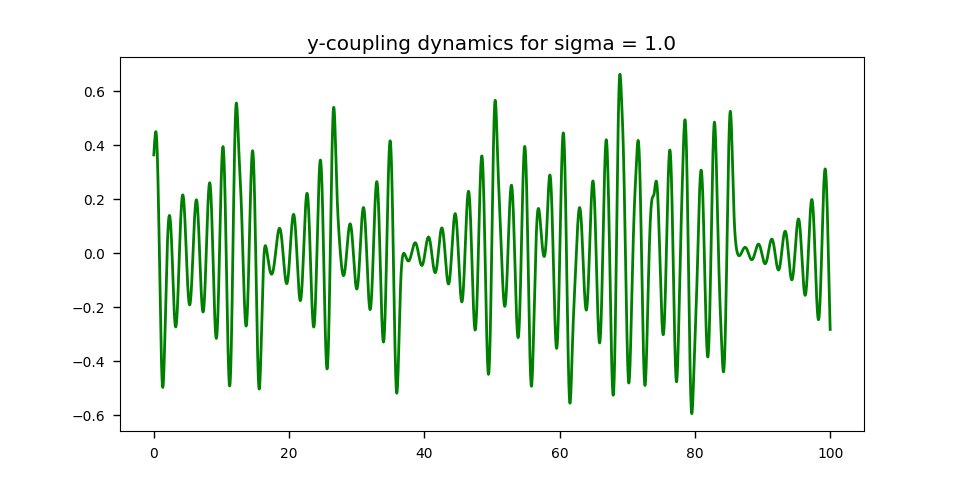
\includegraphics[width = 4in, height = 2in]{y_coupled_y_dynamics_s1.png}
\caption{y component dynamics through time y-y coupling}
\end{figure}

\begin{figure}[H]
\centering
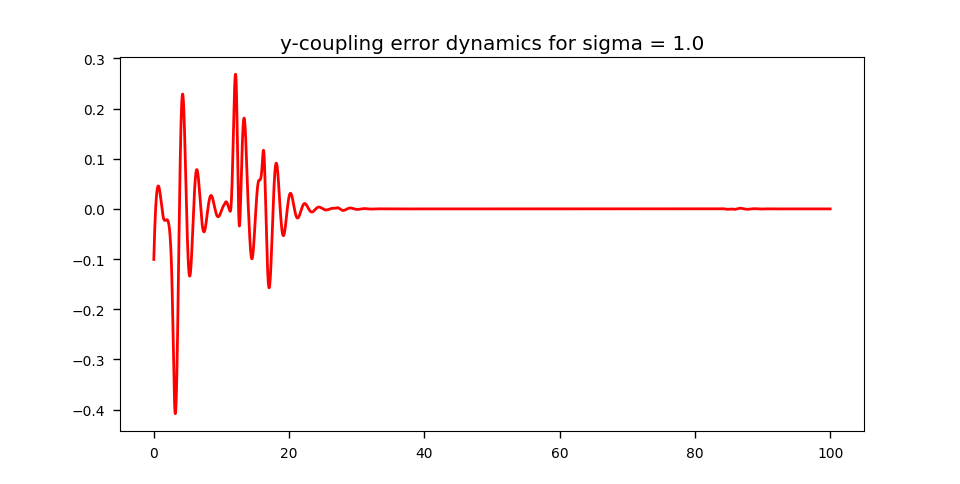
\includegraphics[width = 4in, height = 2in]{y_coupled_y_error_s1.png}
\caption{y component error dynamics through time y-y coupling}
\end{figure}

Hence the system exhibits stable synchronisation for $\sigma >\approx 1$

\begin{figure}[H]
\centering
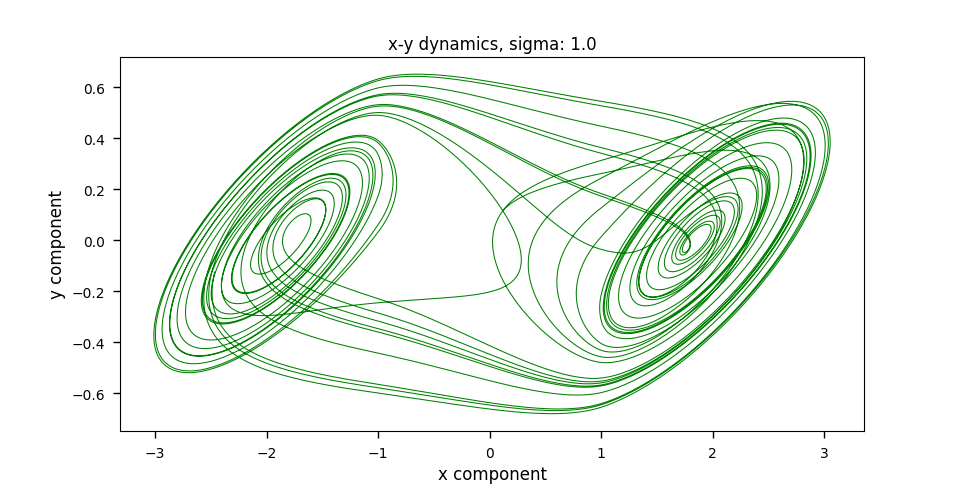
\includegraphics[width = 4in, height = 2in]{y_coupled_s1_xy.png}
\caption{x - y dynamics for the y - y coupling}
\end{figure}

\begin{figure}[H]
\centering
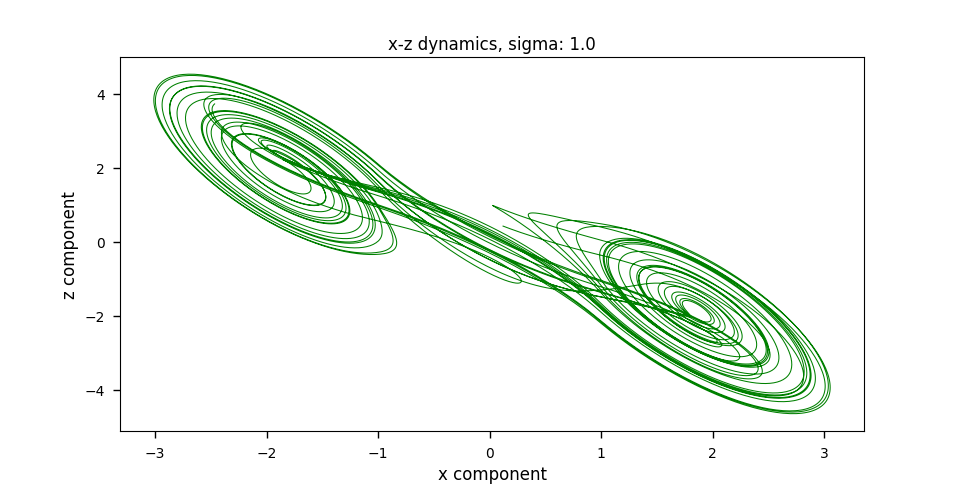
\includegraphics[width = 4in, height = 2in]{y_coupled_s1_xz.png}
\caption{x - z dynamics for the y - y coupling}
\end{figure}

\begin{figure}[H]
\centering
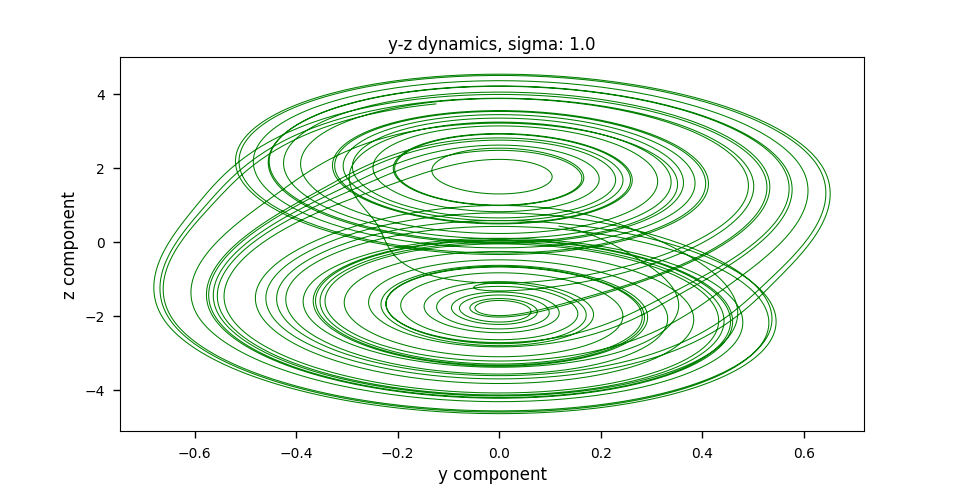
\includegraphics[width = 4in, height = 2in]{y_coupled_s1_yz.png}
\caption{y - z dynamics for the y - y coupling}
\end{figure}

The error dynamics in the z-z coupled system converged for all values of $\sigma < 9$ (approx). any small increase in the
coupling strength past approximately 9 lead to a dramatic change in the error dynamics.
For example, the z-z dynamics for $\sigma = 10.0$ blew up to $-\infty$ while the error for $\sigma = 10.1$ blew up to $\infty$

\begin{figure}[H]
\centering
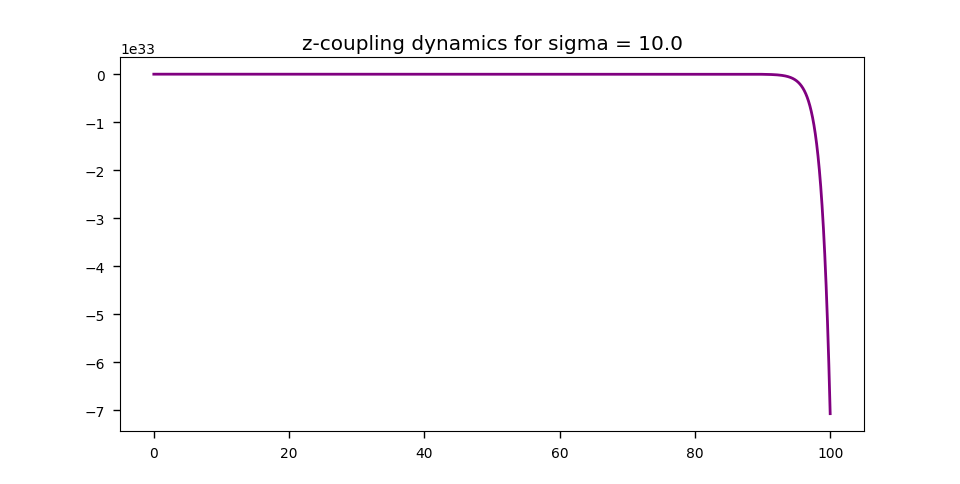
\includegraphics[width = 4in, height = 2in]{z_coupling_z_dynamics_s10.png}
\caption{z component dynamics through time, z-z coupling}
\end{figure}

\begin{figure}[H]
\centering
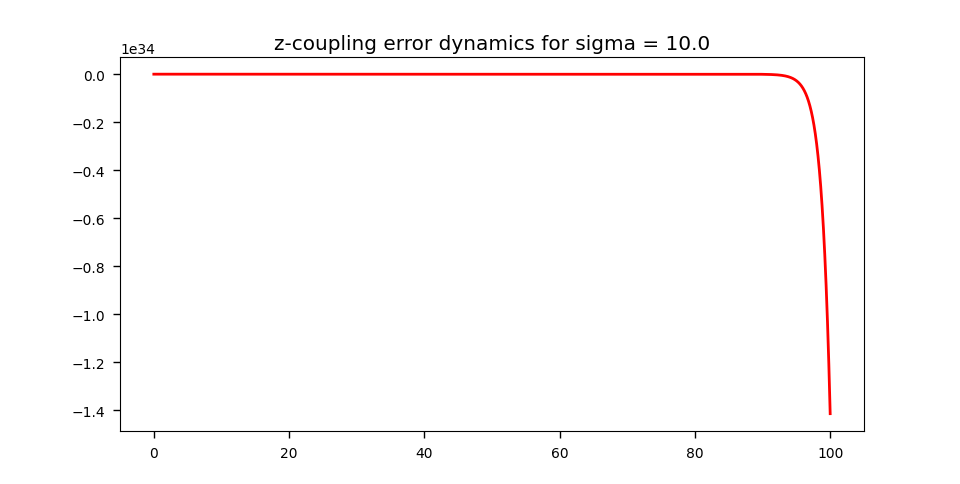
\includegraphics[width = 4in, height = 2in]{z_coupling_z_error_s10.png}
\caption{z component error dynamics through time, z-z coupling}
\end{figure}

\begin{figure}[H]
\centering
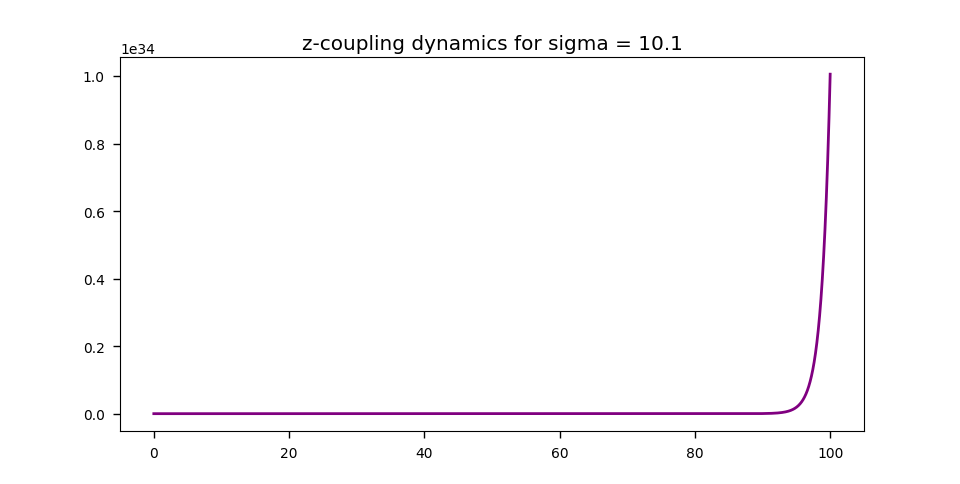
\includegraphics[width = 4in, height = 2in]{z_coupling_z_dynamics_s101.png}
\caption{z component dynamics through time, z-z coupling}
\end{figure}

\begin{figure}[H]
\centering
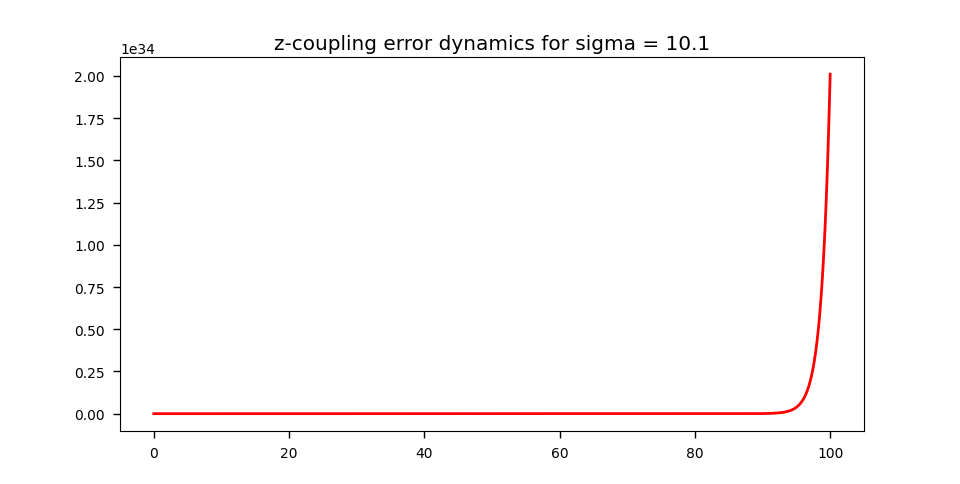
\includegraphics[width = 4in, height = 2in]{z_coupling_z_error_s101.png}
\caption{z component error dynamics through time, z-z coupling}
\end{figure}

Hence the system exhibits stable synchronisation for $\sigma \approx 1$. Indeed we have:

\begin{figure}[H]
\centering
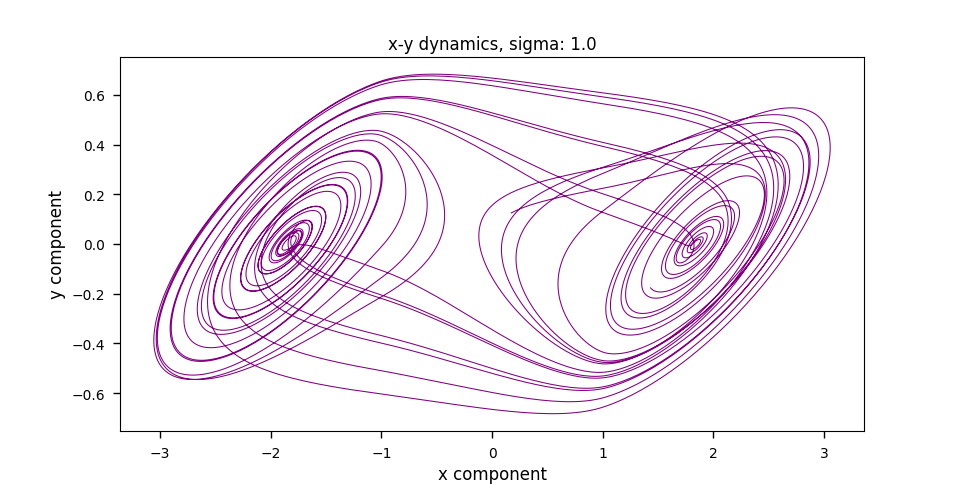
\includegraphics[width = 4in, height = 2in]{z_coupling_xy.png}
\caption{x-y dynamics for the z-z coupling}
\end{figure}

\begin{figure}[H]
\centering
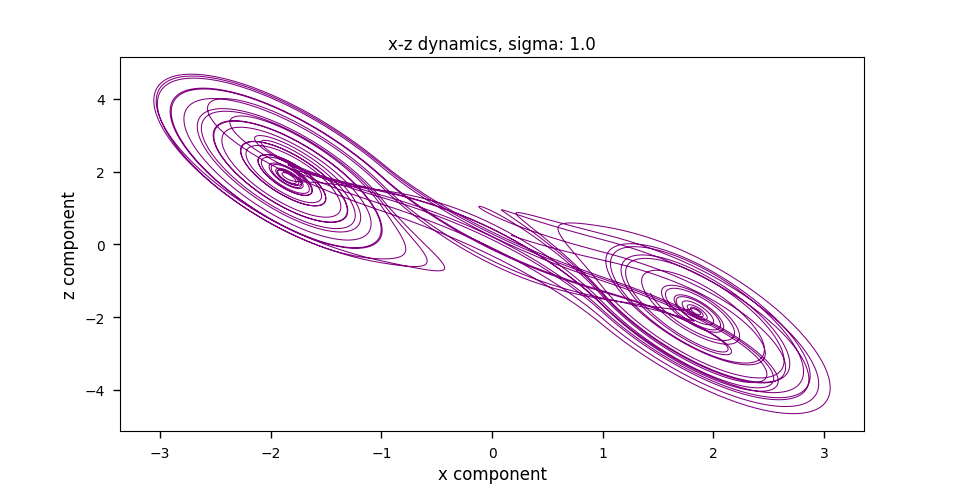
\includegraphics[width = 4in, height = 2in]{z_coupling_xz.png}
\caption{x-z dynamics for the z-z coupling}
\end{figure}

\begin{figure}[H]
\centering
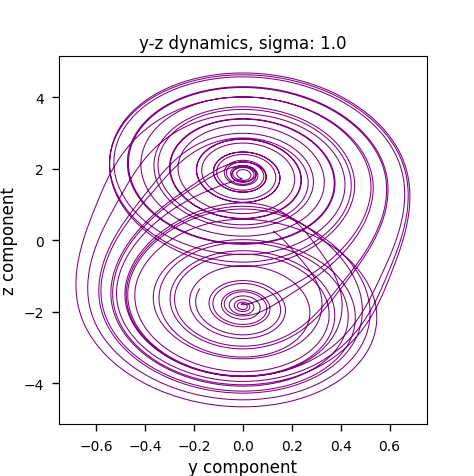
\includegraphics[width = 4in, height = 2in]{z_coupling_yz.png}
\caption{y-z dynamics for the z-z coupling}
\end{figure}

For which the corresponding error dynamics in the z component is:

\begin{figure}[H]
\centering
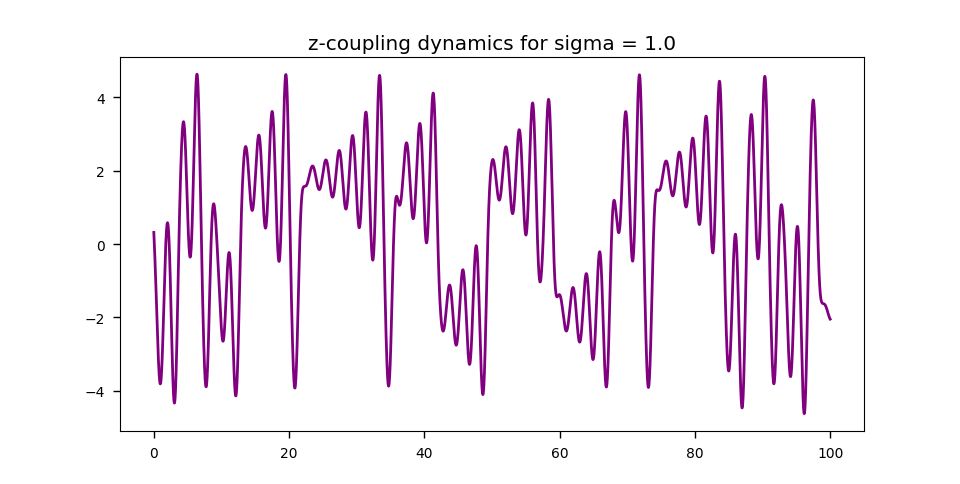
\includegraphics[width = 4in, height = 2in]{z_coupling_z_dynamics_s1.png}
\caption{z component dynamics through time z-z coupling}
\end{figure}

\begin{figure}[H]
\centering
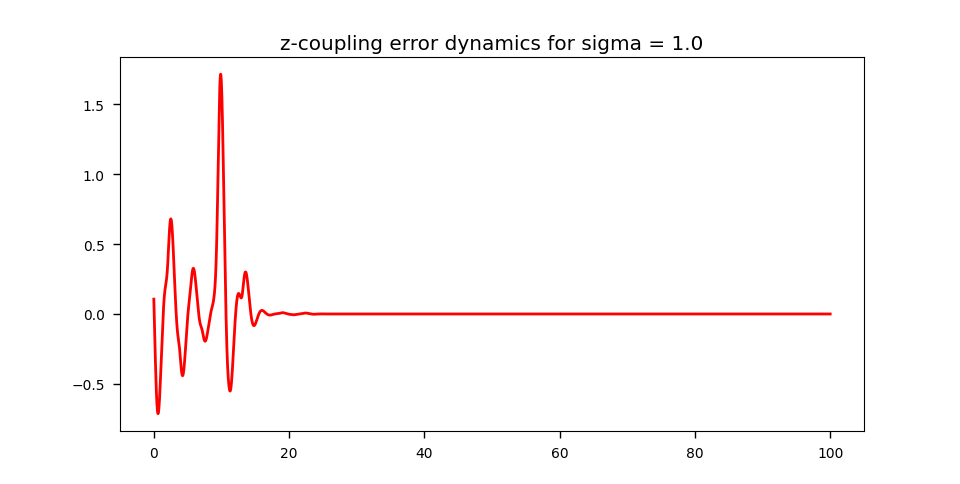
\includegraphics[width = 4in, height = 2in]{z_coupling_z_error_s1.png}
\caption{z component error dynamics through time z-z coupling}
\end{figure}




\subsection*{Question 2}
The maths for question 2
The following is a graph:


\subsection*{Question 3}
Maths for question 3


\end{document}
